\begin{frame}{Extrapolation to Run-3}
\begin{columns}
\column{0.5\textwidth}
\begin{itemize}
    \item Scale Run-2 with 300/139 $\sim$ 2.16
    \item Expected 95\% CL limit on $\sigma_{HH}$ of 3.3
    \item $\mu_{HH} = 1 \pm 1.52$ for SM
    \item SM HH significance: 0.71$\sigma$ 
\end{itemize}

\column{0.5\textwidth}
\begin{figure}
    \centering
    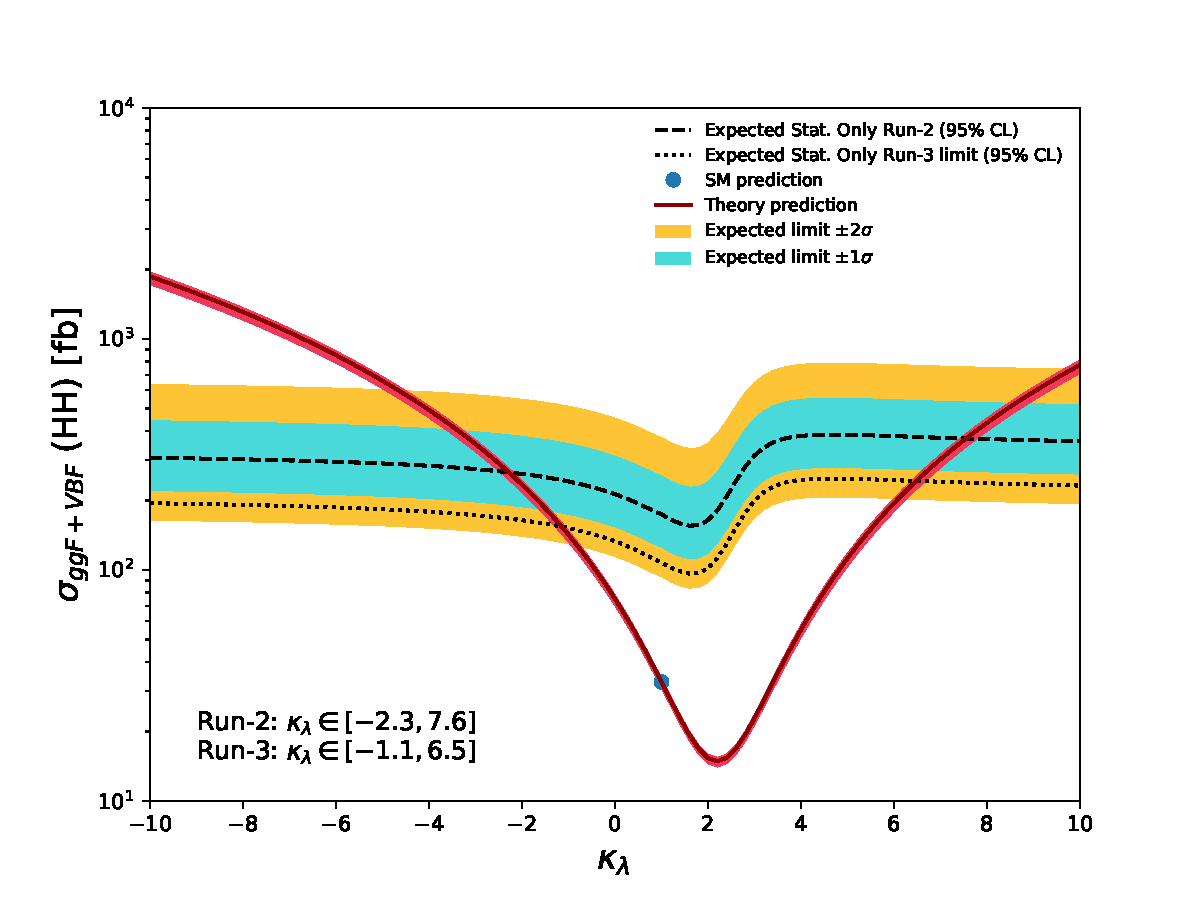
\includegraphics[width=1.\textwidth]{BackUp/Part4/Img/kappa_lambda_Run_3_stat.pdf}
\end{figure}
\end{columns}    
\end{frame}

\begin{frame}{European strategy}
\begin{columns}
\column{0.5\textwidth}
\begin{itemize}
    \item Monte Carlo based $b\bar{b}\gamma\gamma$ analysis
    \item One BDT category, 40\% efficiency and 99\% of background rejection
    \item Signal extracted using $m_{b\bar{b}\gamma\gamma}$ variable.
    \item $\mu = 1 \pm 0.6$ with significance of 2.1$\sigma$
\end{itemize}

\begin{figure}
    \centering
    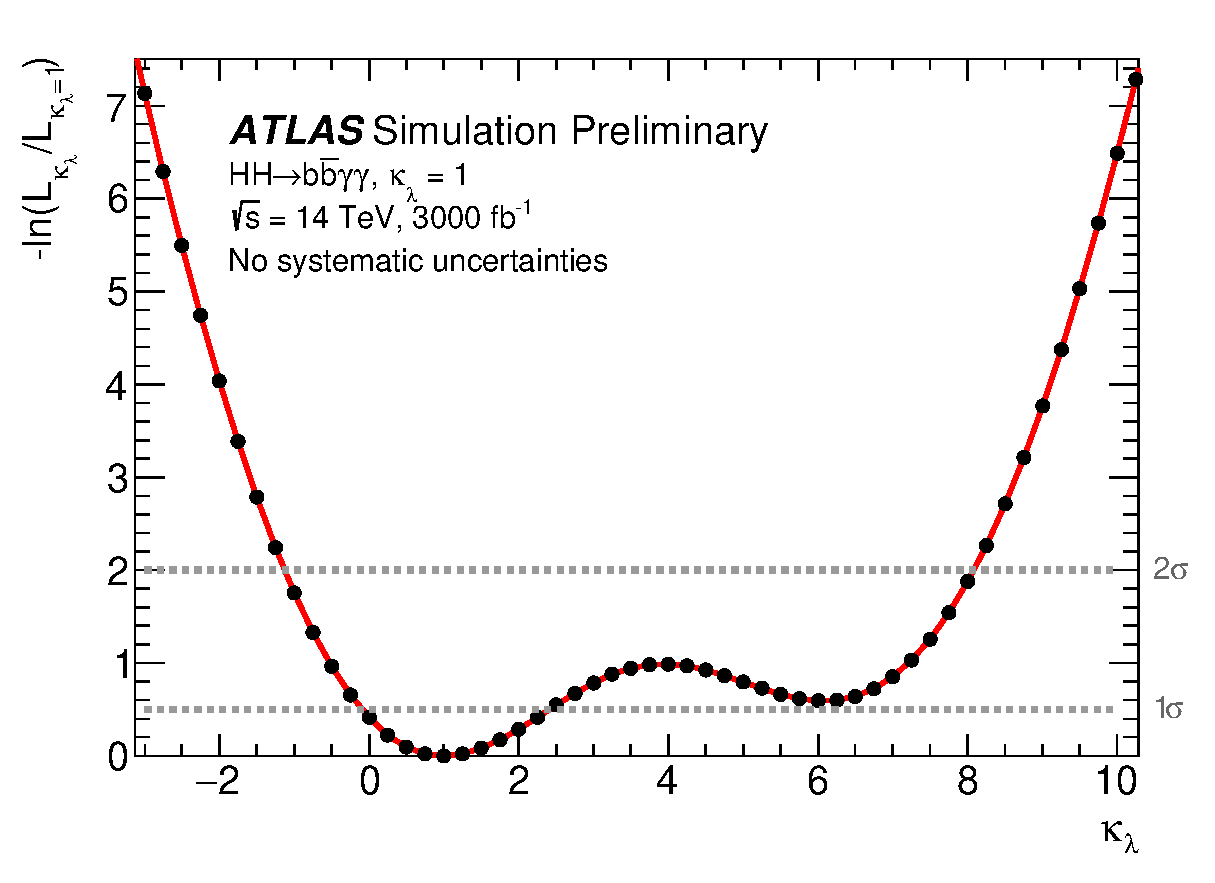
\includegraphics[width=1.\textwidth]{BackUp/Part4/Img/figures_bbyy_NoSyst_likelihoodCurve_-3to10.eps}
\end{figure}

\column{0.5\textwidth}
\begin{figure}
    \centering
    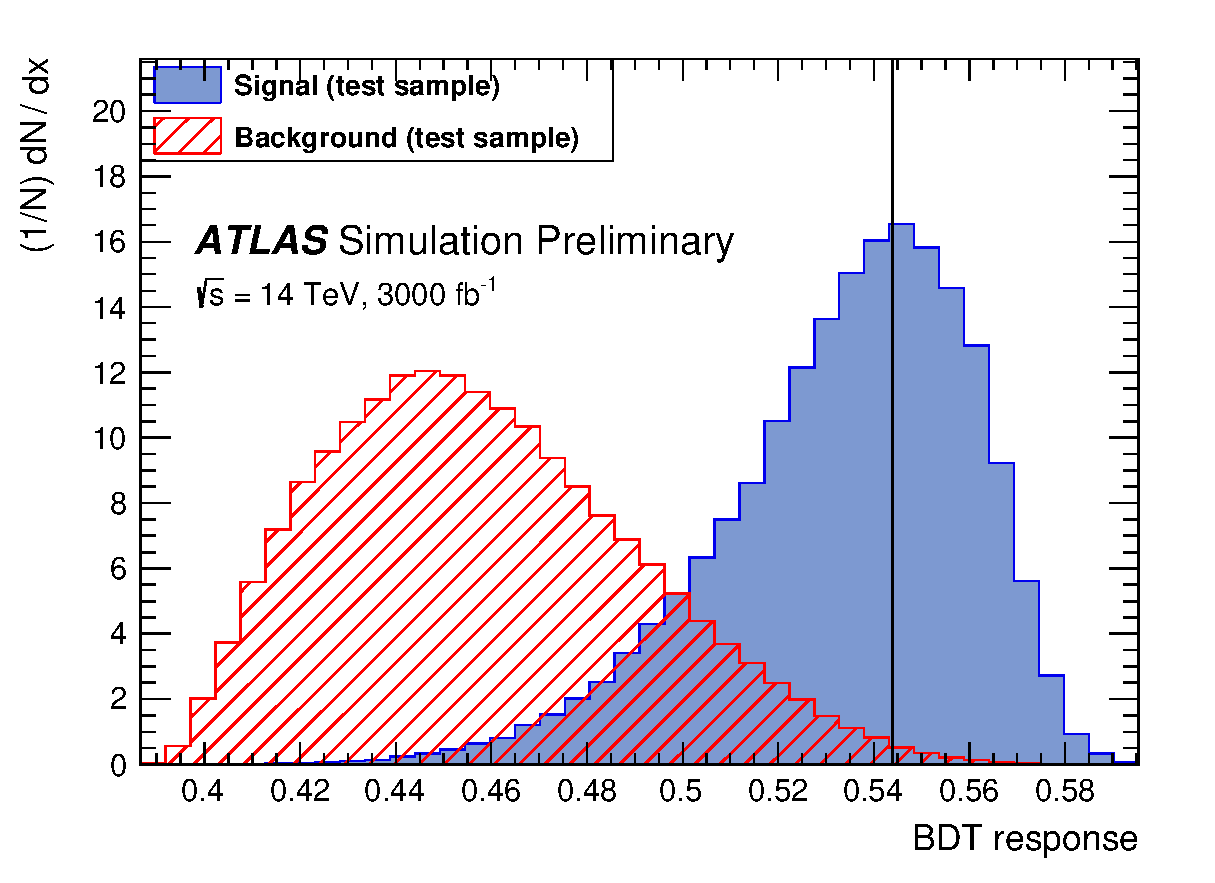
\includegraphics[width=.9\textwidth]{BackUp/Part4/Img/figures_bbyy_overtrainTestOnly.eps}
\end{figure}

\begin{table}[htbp]
    \centering
    \begin{tabular}{lcc}
\hline \hline Scenario & $1 \sigma \ \mathrm{CI}$ & $2 \sigma \ \mathrm{CI}$ \\
\hline Stat. & $-0.1<\kappa_{\lambda}<2.4$ & $-1.1<\kappa_{\lambda}<8.1$ \\
Syst. & $-0.2<\kappa_{\lambda}<2.5$ & $-1.4<\kappa_{\lambda}<8.2$ \\
\hline \hline
\end{tabular}
\end{table}
\end{columns}    
\end{frame}
\begin{frame}{Extrapolation to HL-LHC}
\begin{table}[htbp]
    \centering
    \begin{tabular}{lcccccccccc}
    \hline\hline
    Process & ggF HH & VBF HH & ggF H & VBF H & $t\bar{t}$H & WH & ZH & tHjb & tWH & $\gamma\gamma$\\
    \hline
    Scale & 1.19 & 1.2 & 1.13 & 1.13 & 1.21 & 1.1 & 1.11 & 1.21 & 1.22 & +18\% \\
    \hline\hline
    \end{tabular}
\end{table}

\begin{table}[htbp]
    \centering
    \begin{tabular}{lcc}
    \hline\hline 
        Scenario & Run-2 Stat. Only & HL-LHC Stat. Only \\
    \hline    
        High mass, High BDT & 0.47 & 2.38 \\
        High mass, Low BDT  & 0.13 & 0.64 \\
        Low mass, High BDT  & 0.03 & 0.15 \\
        Low mass, Low BDT   & 0.02 & 0.10 \\
        \hline
        Combined & 0.48$\sigma$ & 2.47$\sigma$ \\
    \hline\hline 
    \end{tabular}
\end{table}

\begin{itemize}
    \item $\mu_{HH} = 1 \pm 0.44$
\end{itemize}

\end{frame}

\begin{frame}{Prospect in FCC-hh}
\href{https://arxiv.org/abs/2004.03505}{2004.03505}
\begin{columns}
\column{0.5\textwidth}
\begin{itemize}
    \item $pp$ collider at $\sqrt{s} = $ 100 TeV.
    \item $\mathcal{L}_{int} = $ 30 ab$^{-1}$
    \item From 14 TeV to 100 TeV, $\times$ 30 increase in cross-section 
\end{itemize}

\begin{figure}
    \centering
    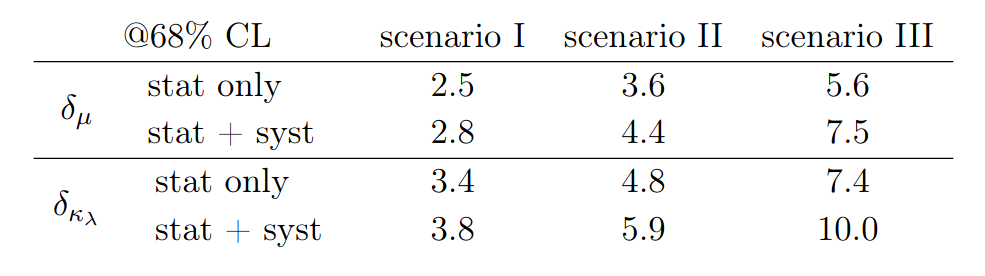
\includegraphics[width=0.8\textwidth]{BackUp/Part4/Img/kl_1sigma_FCC.png}
\end{figure}

\begin{itemize}
    \item Sensitivity driven by $b\bar{b}\gamma\gamma$
    \item \textbf{Systematics limited}  (control of systematic needed) 
\end{itemize}

\column{0.5\textwidth}

\begin{figure}
    \centering
    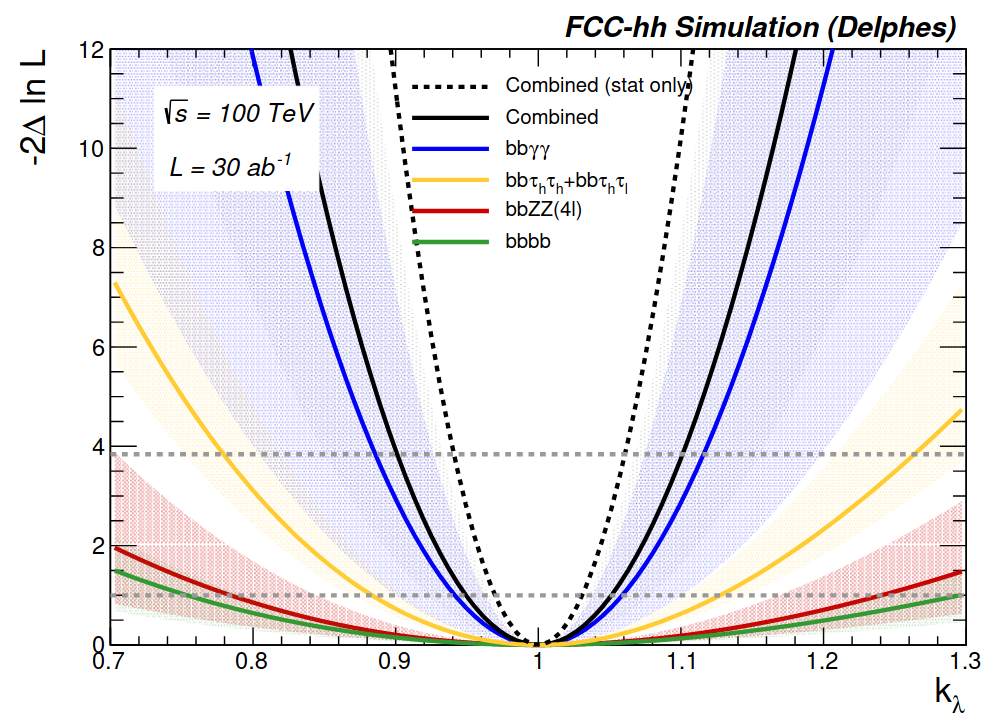
\includegraphics[width=0.8\textwidth]{BackUp/Part4/Img/kl_comb_FCC.png}
\end{figure}

\begin{itemize}
    \item Scenario I: optimistic, detector performance similar to Run-2
    \item Scenario II: realistic, intermediate
    \item Scenario III: conservative (pessimistic), extrapolated from HL-LHC performances 
\end{itemize}

\end{columns}
\end{frame}
\begin{frame}{Systematics scenarios}
\begin{figure}
    \centering
    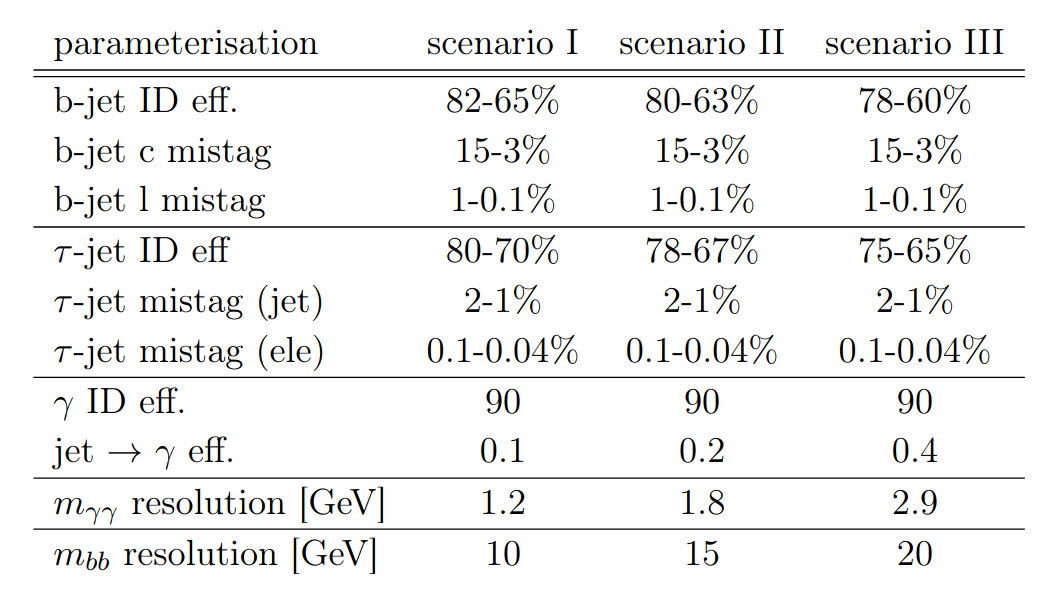
\includegraphics[width=0.8\textwidth]{BackUp/Part4/Img/Sys_FCC.png}
\end{figure}
\end{frame}

\begin{frame}{Prospect in $e^{+}e^{-}$ collider}
\begin{columns}
\column{0.5\textwidth}
\begin{itemize}
    \item directly accessible via ZHH and $\nu\bar{\nu}$HH
    \item $\delta^{\text{ILC}}$(1 TeV) = 10\% , $\delta^{\text{CLIC}}$(3 TeV) = 9\%
\end{itemize}

\column{0.5\textwidth}
\begin{figure}
    \centering
    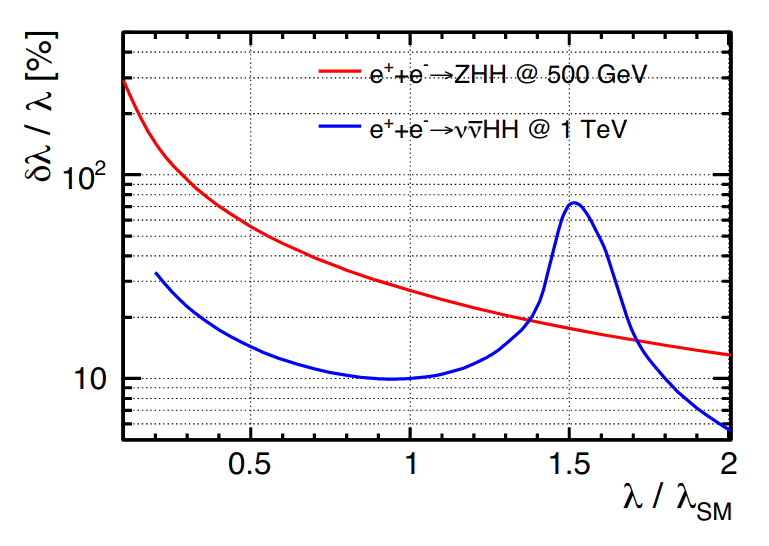
\includegraphics[width=0.8\textwidth]{BackUp/Part4/Img/kl_preci_ILC.png}
\end{figure}

\end{columns}
\end{frame}

\begin{frame}{Knowledge from $\kappa_{\lambda}$}
\begin{columns}
\column{0.5\textwidth}
\begin{itemize}
    \item \textbf{50\% sensitivity} $\to$ reject $\kappa_{\lambda}$ = 0 at 95\%
    \item \textbf{20\% sensitivity} $\to$ 5$\sigma$ discovery of SM HH
    \item \textbf{5\% sensitivity} $\to$ sensitive to quantum corrections to Higgs potential
\end{itemize}

\begin{itemize}
    \item Precise measurement of $\kappa_{\lambda}$ at FCC-hh requires precise knowledge of $\kappa_{t}$ 
    \item 1\% $\kappa_{t}$ leads to 5\% $\kappa_{\lambda}$
    \item precise measurement of $\kappa_{t}$ needs FCC-ee
\end{itemize}

\column{0.5\textwidth}
\begin{figure}
    \centering
    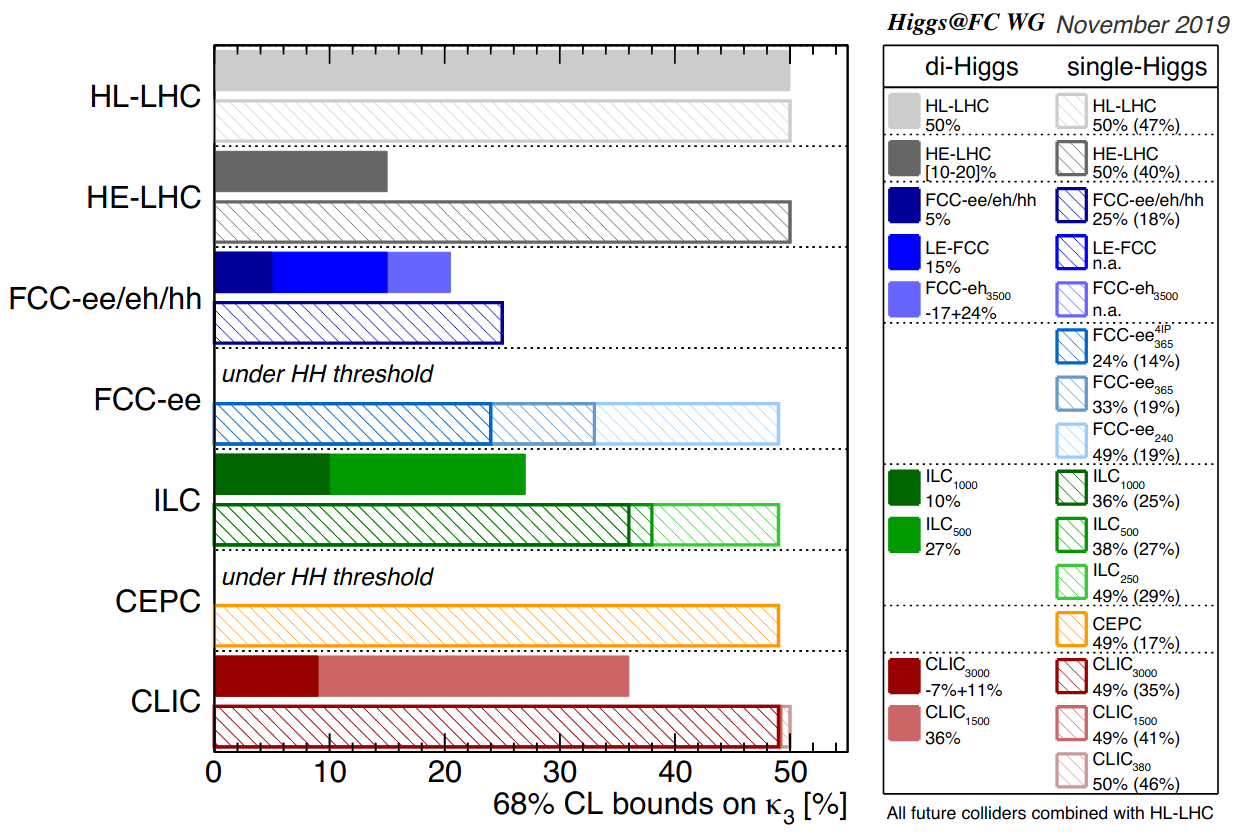
\includegraphics[width=1.\textwidth]{BackUp/Part4/Img/kl_future_C.png}
\end{figure}
\end{columns}
\end{frame}